% !TeX program = xelatex
% ============================================================================
%  AICoding考试平台 软件需求规格说明 —— 初稿（填写中）
%
%  结构说明：
%    参考课程往年样例 2：项目背景与目标、典型用户与痛点、
%    需求分析、用户故事地图与故事卡、系统架构、迭代计划。
%
%  编译方式：
%    1. 必须使用 XeLaTeX 编译，不要使用 pdfLaTeX。
%    2. 推荐命令：xelatex requirements_v2.tex
%    3. Overleaf：Menu -> Compiler -> XeLaTeX
%    4. 如果出现中文字体错误，将 documentclass 行改为：
%       \documentclass[UTF8,12pt,a4paper,fontset=fandol]{ctexart}
% ============================================================================

\documentclass[UTF8,12pt,a4paper]{ctexart}

\usepackage{geometry}
\geometry{left=2.6cm,right=2.6cm,top=2.8cm,bottom=2.8cm}
\usepackage{booktabs}
\usepackage{longtable}
\usepackage{tabularx}
\usepackage{array}
\usepackage{enumitem}
\usepackage{graphicx}
\usepackage{float}
\usepackage{caption}
\usepackage{xcolor}
\usepackage{fancyhdr}
\usepackage{makecell}
\usepackage{amsmath}
\usepackage{amssymb}
\usepackage{setspace}
\usepackage{url}
\usepackage[hidelinks]{hyperref}

\linespread{1.35}
\setlength{\parindent}{2em}
\setlength{\parskip}{0.25em}
\renewcommand{\arraystretch}{1.25}
\newcolumntype{L}[1]{>{\raggedright\arraybackslash}p{#1}}
\newcolumntype{Y}{>{\raggedright\arraybackslash}X}
\newcommand{\fillme}[1]{\textcolor{red}{#1}}
\newcommand{\placeholder}[1]{\textcolor{red}{【#1】}}

% 生僻字回退字体：优先 Noto Serif CJK SC，其次 AR PL UMing CN，最后 FandolSong。
% 用于“刘璘”等 Fandol 字库可能缺失的字符。
\IfFontExistsTF{Noto Serif CJK SC}{
  \newCJKfontfamily\rarefont{Noto Serif CJK SC}
}{
  \IfFontExistsTF{AR PL UMing CN}{
    \newCJKfontfamily\rarefont{AR PL UMing CN}
  }{
    \newCJKfontfamily\rarefont{FandolSong}
  }
}

\pagestyle{fancy}
\fancyhf{}
\fancyhead[L]{\small AICoding考试平台需求规格说明}
\fancyhead[R]{\small V1.0}
\fancyfoot[C]{\thepage}
\renewcommand{\headrulewidth}{0.4pt}

\begin{document}

% ============================================================================
% 封面
% ============================================================================
\begin{titlepage}
\thispagestyle{empty}
\centering
\vspace*{1.5cm}

{\Large 清华大学\par}
\vspace{0.4cm}
{\large 软件工程\par}

\vspace{2.2cm}
{\Huge\bfseries 软件需求规格说明\par}
\vspace{0.8cm}
{\LARGE AICoding考试平台\par}

\vspace{2.0cm}
\begin{tabular}{rl}
文档版本：& V1.0 \\
文档日期：& 2026-10-23 \\
项目组：& A10 组 \\
小组成员：& 康祥桢、石恒睿、吕浩、李劲逸 \\
课程教师：& 刘\rarefont{璘} \\
\end{tabular}

\vfill
{\small 本文档参考课程往年样例的结构组织。\par}
\end{titlepage}

% ============================================================================
% 修改历史与目录
% ============================================================================
\section*{修改历史}
\addcontentsline{toc}{section}{修改历史}

\begin{table}[H]
\centering
\begin{tabularx}{\textwidth}{|p{2.6cm}|p{1.8cm}|Y|p{2.6cm}|}
\hline
\textbf{日期} & \textbf{版本} & \textbf{说明} & \textbf{作者} \\ \hline
2026-10-23 & V1.0 & 初稿 & \\ \hline
 & & & \\ \hline
\end{tabularx}
\end{table}

\newpage
\tableofcontents
\newpage

% ============================================================================
% 1 项目背景和项目目标
% ============================================================================
\section{项目背景和项目目标}

\subsection{项目背景}

AI 编程工具正在成为软件开发的默认方式。Copilot、Cursor、Claude Code 等工具能够读取代码仓库、修改多个文件、运行测试，“会不会用 AI 编程”正在成为新的能力分水岭。但传统在线评测系统（OJ）仍以“最终代码是否通过隐藏用例”作为主要信号；大量题目已经进入模型训练数据，AI 可以直接给出答案，分数的区分度越来越低。简单禁用 AI 又与真实工作方式脱节，且难以执行。

更根本的是，OJ 只记录最终提交，看不到解题过程。学生如何拆解问题、选择方案、设计测试、调试错误、判断 AI 建议是否可信，这些真正体现工程能力的行为都没有留下证据。结果是“能跑通、讲不清”可以稳定拿到高分，教师也无法判断一份代码是独立完成、AI 生成还是他人代写。

通用 AI 编程助手能辅助编码，却不能承担考试职能：它们没有隔离环境、统一镜像、限时/次数/资源约束、隐藏测试与判分，也没有可审计的过程记录。企业技术面试同样缺少一种能同时观察候选人编码能力、AI 协作能力和验证过程的工具。因此，本产品把 Agent、考试机制与过程性评价结合起来：在隔离容器中提供 IDE、终端和 Coding Agent，记录 AI 对话、代码快照、命令和测试结果，用样例/隐藏测试判分，用过程报告和申诉证据让评价可解释。

\subsection{产品定位与竞品分析}

本产品是一个以 Agent 交互为特色、以过程性评价为核心的 AICoding考试平台：考生在隔离容器中通过 IDE、终端和 Agent 完成工程任务，平台记录 AI 对话、代码快照、命令和测试结果，用样例/隐藏测试判分，并生成过程报告。

与 LeetCode、牛客、Copilot、ChatGPT 相比，本产品的差异不是题库更多或 Agent 更聪明，而是把“真实开发环境 + 考试治理 + 过程证据”放在同一个系统里。

\begin{table}[H]
\centering
\caption{竞品综合对比}
\label{tab:competitors}
\small
\begin{tabularx}{\textwidth}{|p{2.2cm}|Y|Y|Y|}
\hline
\textbf{维度} & \textbf{LeetCode / 牛客（OJ 类）} & \textbf{Copilot / ChatGPT（AI 助手类）} & \textbf{本产品} \\ \hline
题目形态 & 单文件算法题、笔试题 & 任意代码、对话 & 工程题（初始仓库）+ 可选算法题 \\ \hline
作答环境 & 浏览器编辑器 & 本地 IDE 或聊天窗口 & 隔离容器 + 浏览器 IDE + 终端 \\ \hline
AI 辅助 & 无或禁用 & 有，但无考试约束 & 有，受控、可配置、全程留痕 \\ \hline
判分方式 & 隐藏用例、笔试评分 & 无 & 样例 + 隐藏用例 + 过程报告 \\ \hline
过程记录 & 仅最终提交 & 仅本地代码或对话 & AI 对话/代码快照/命令/测试/提交 \\ \hline
考试治理 & 有限 & 无 & 限时/次数/资源/审计 \\ \hline
适用场景 & 刷题、初筛、笔试 & 日常开发、学习 & 课程考试、面试、认证 \\ \hline
\end{tabularx}
\end{table}

\subsection{项目目标}

本产品的目标是：在隔离的类真实开发环境中，用 Agent 交互、考试机制和过程性评价，测量考生“会不会用 AI 写好代码”，并输出可解释的能力报告。

具体包括：
\begin{itemize}[leftmargin=2em]
  \item \textbf{真实：}隔离容器、IDE、终端和 Agent；
  \item \textbf{受控：}限时、提交次数、资源限制、AI 策略和操作留痕；
  \item \textbf{可解释：}测试结果、过程报告、时间线和申诉证据。
\end{itemize}

课程考试场景下，目标是恢复区分度、降低判分负担；面试场景下，目标是用工程题观察候选人的拆解、验证和审查 AI 的能力。首期按 30--60 人/场设计，容器启动 $<$ 60 秒，单次判分 $<$ 2 分钟。

\textbf{非目标：}不做题库市场、不做完整 IDE、不自研大模型、首期不做多租户、不做侵入式监控。

\section{典型用户分析和用户痛点问题}

\subsection{应用场景}

本产品主要面向软件工程类课程的考试与训练，也可扩展到企业面试和技术认证。典型流程是：教师创建考试与题目、配置评分规则与 Agent 策略；考生在隔离容器中通过 IDE、终端和 Agent 完成任务；系统自动判分并生成过程报告；教师复核成绩，学生申诉。

主要场景：课程机考（P0）；企业面试初筛（P1）；随堂训练和技术认证（P2）。

\subsection{用户类型}

\begin{itemize}[leftmargin=2em]
  \item \textbf{学生（考生）：}软件工程类课程在读学生，有编程基础；关注环境稳定、规则透明、能展示 AI 协作、获得可解释反馈。
  \item \textbf{教师（含命题人、监考/助教、面试官）：}授课教师、助教或企业技术面试官，负责出题、配评分、监考、面试和分析；关注题目能测真实能力、过程可见、判分负担低，以及面试信号客观可比。
  \item \textbf{平台管理员：}负责运维、权限、数据安全和系统配置；关注稳定、隔离、可审计。
\end{itemize}

\subsection{用户痛点}

学生痛点主要来自 18 份问卷的选择题与开放题结果（详见附录调研记录）；教师与管理员痛点来自竞品分析和产品分析。

\subsubsection{学生（考生）}

\begin{itemize}[leftmargin=2em]
  \item \textbf{环境不一致：}本地 IDE、依赖和网络差异，导致“非能力性失败”。
  \item \textbf{规则不清：}AI 能不能用、用到什么程度，缺少可执行说明。
  \item \textbf{过程不可见：}只看最终代码，无法展示拆解、验证和调试；只有分数，没有改进反馈。
  \item \textbf{考核与真实开发脱节：}问卷中 7/18 认为现有考核侧重算法技巧或语法记忆，较少涉及实际项目问题。
  \item \textbf{AI 代码难以判断与解释：}14/18 表示代码能跑但难以判断实现是否正确、可靠；11/18 表示难以解释 AI 生成的关键逻辑。
\end{itemize}

\subsubsection{教师（含命题、监考、面试场景）}

\begin{itemize}[leftmargin=2em]
  \item \textbf{题目被 AI 秒杀：}题目进入训练数据，AI 直接给答案，分数失去区分度。
  \item \textbf{过程不可见：}无法判断学生或候选人是否理解、是否会验证和调试。
  \item \textbf{判分负担大：}过程性评价人力成本高，考务工具割裂。
  \item \textbf{面试信号失真：}算法题和笔试无法区分“会写代码”和“会用 AI 写好代码”；面试成本高、评分标准不一，缺少可对比报告。
  \item \textbf{监考与取证困难：}环境准备、异常发现和申诉取证依赖人工，缺少统一的时间线和证据链。
\end{itemize}

\subsubsection{平台管理员}

\begin{itemize}[leftmargin=2em]
  \item \textbf{容器与镜像管理复杂：}每人一个容器，镜像、依赖、配额和回收需要统一管理。
  \item \textbf{隔离与安全：}容器、判题服务和外部网络之间需要严格隔离。
  \item \textbf{权限与审计：}多角色、多课程、多场景，功能权限、数据范围和审计合规压力大。
\end{itemize}

\subsection{痛点根因与产品回应}

这些痛点的共同根因是：最终代码不等于能力，过程没有被记录，AI 使用规则不可执行。产品回应是把 AI 对话、代码快照、命令和测试记录成过程证据，用测试用例 + 教师复核做评价。

\section{需求分析}

\subsection{调研方法及需求规格书信息表}

\subsubsection{调研方法}

\begin{itemize}[leftmargin=2em]
  \item \textbf{竞品分析：}分析 LeetCode、牛客、Copilot、ChatGPT 的判题、AI 辅助和考试流程。
  \item \textbf{问卷调查：}面向软件工程类课程学生发放问卷，回收 18 份，覆盖现有考核不足、AI 编程问题、期望的考核任务/能力/工作台功能。
  \item \textbf{原型设计与走查：}设计三栏界面，检查容器、编辑器、Agent 和判分流程。
\end{itemize}

\subsubsection{需求规格书信息表}

\begin{table}[H]
\centering
\small
\begin{tabularx}{\textwidth}{|p{4.0cm}|Y|}
\hline
\textbf{项目} & \textbf{内容} \\ \hline
需求作者 & A10 组 \\ \hline
需求实现责任人 & A10 组 \\ \hline
需求来源 & 问卷调研、竞品分析、原型设计 \\ \hline
需求优先级 & 高 \\ \hline
需求状态 & 初稿 \\ \hline
相关需求 & 无 \\ \hline
需求版本号 & V1.0 \\ \hline
系统版本号 & V0.1 \\ \hline
\end{tabularx}
\end{table}

\subsection{用户类型与权限}

平台分学生、教师、管理员三类角色。教师角色覆盖命题人、监考/助教和面试官三种职责，通过权限范围区分课程考试与企业面试场景；学生只能进入本人考试、查看本人报告；教师可以创建考试、查看本班成绩和过程记录，面试场景下只能查看受邀候选人；管理员负责账号、权限、镜像和审计。关键操作写入审计日志。

\begin{table}[H]
\centering
\caption{角色与权限矩阵}
\label{tab:permissions}
\small
\begin{tabularx}{\textwidth}{|Y|p{1.6cm}|p{2.2cm}|p{1.8cm}|}
\hline
\textbf{功能} & \textbf{学生} & \textbf{教师} & \textbf{管理员} \\ \hline
查看考试与须知 & $\checkmark$ & $\checkmark$ & $\checkmark$ \\ \hline
创建/编辑考试与任务 & -- & $\checkmark$ & $\checkmark$ \\ \hline
配置测试、AI 策略与资源 & -- & $\checkmark$ & $\checkmark$ \\ \hline
进入隔离容器作答 & $\checkmark$ & -- & -- \\ \hline
使用 Coding Agent & $\checkmark$ & -- & -- \\ \hline
提交判分 & $\checkmark$ & -- & -- \\ \hline
查看本人成绩与报告 & $\checkmark$ & $\checkmark$ & $\checkmark$ \\ \hline
查看班级成绩与过程记录 & -- & $\checkmark$ & $\checkmark$ \\ \hline
监考处置、补时与复核申诉 & -- & $\checkmark$ & $\checkmark$ \\ \hline
面试管理与候选人报告 & -- & $\checkmark$ & $\checkmark$ \\ \hline
账号、镜像、审计与系统配置 & -- & -- & $\checkmark$ \\ \hline
\end{tabularx}
\end{table}

\subsection{功能需求}

\subsubsection{用户与权限管理}

\textbf{需求描述：}支持学生、教师、管理员的账号和权限管理；教师角色内再按命题、监考、面试职责细分权限。

\begin{enumerate}[leftmargin=2em,itemsep=2pt]
  \item \textbf{账号管理。}管理员创建、编辑账号，批量导入学生名单和面试候选人名单；名单支持 CSV/Excel，校验学号/姓名/邮箱格式，导入结果给出成功/失败明细。
  \item \textbf{角色权限。}学生、教师、管理员三类角色；教师按命题人、监考/助教、面试官职责配置功能权限，并按数据范围（本人/本班/受邀候选人/全部）授权。
  \item \textbf{登录与审计。}支持登录、找回密码；登录、权限变更和关键操作写入审计日志。
\end{enumerate}

\subsubsection{题库与考试管理}

\textbf{需求描述：}支持题目创建、测试用例管理，以及考试创建、组卷、发布和归档。

\begin{enumerate}[leftmargin=2em,itemsep=2pt]
  \item \textbf{题目管理。}创建工程题或算法题，填写题面、初始仓库、依赖镜像和测试用例；样例测试对学生可见，隐藏测试不可见。
  \item \textbf{创建考试。}填写名称、时间、时长、提交次数和 AI 使用策略，保存为草稿。
  \item \textbf{组卷与评分规则。}从题库选题，设置分值、测试用例权重、过程分权重和及格线。
  \item \textbf{发布与归档。}支持发布、撤回、开始、结束和归档；发布前校验时间、名单、题目和测试完整性。
\end{enumerate}

\subsubsection{隔离环境与代码编辑}

\textbf{需求描述：}为每位考生提供隔离容器和浏览器 IDE，支持编辑、运行、调试和版本回溯。

\begin{enumerate}[leftmargin=2em,itemsep=2pt]
  \item \textbf{容器分配。}按名单为每位考生启动隔离容器，预装课程依赖和初始仓库。
  \item \textbf{文件树与编辑器。}支持打开、新建、修改文件，语法高亮、自动补全和查找替换。
  \item \textbf{终端与运行。}支持执行命令、编译、运行测试，返回输出、退出码和耗时。
  \item \textbf{自动保存与版本回溯。}每 30 秒或每次运行/提交时保存快照；考生可以查看时间线并还原版本。
\end{enumerate}

\subsubsection{Agent 交互}

\textbf{需求描述：}提供受控的编程 Agent，支持多轮对话、提示、追问、代码修改和过程留痕。

\begin{enumerate}[leftmargin=2em,itemsep=2pt]
  \item \textbf{多轮对话。}考生在右侧面板提问，Agent 返回解释、提示或代码建议；支持 @ 文件作为上下文。
  \item \textbf{提示与追问。}根据当前代码和题目给出分层提示、追问思路、引导方案；按策略避免直接给完整答案。
  \item \textbf{代码生成与修改。}生成代码片段或 diff，考生可以采纳、修改或拒绝；按策略允许或禁止直接写入文件。
  \item \textbf{策略与留痕。}教师选择闭卷/提示/建议/协作/自主档位；系统记录 prompt、响应、采纳行为和关联代码版本。
\end{enumerate}

\subsubsection{评分与报告}

\textbf{需求描述：}结合测试用例和过程证据生成成绩、能力报告和改进建议。

\begin{enumerate}[leftmargin=2em,itemsep=2pt]
  \item \textbf{结果评分。}运行样例和隐藏测试，按权重计算代码分；判题失败标记为“需人工复核”。
  \item \textbf{过程评分。}根据 AI 对话、验证行为、调试行为和修改轨迹计算过程分，维度和权重可配置。
  \item \textbf{报告。}展示总分、测试详情、时间线、AI 对话摘要、代码 diff、能力雷达和改进建议。
  \item \textbf{复核与申诉。}教师可以调整过程分、标记争议卷；学生可以在规定时间内申诉。
\end{enumerate}

\subsubsection{监控与训练}

\textbf{需求描述：}支持考试过程监控、异常预警、历史分析，以及非考试场景下的训练模式。

\begin{enumerate}[leftmargin=2em,itemsep=2pt]
  \item \textbf{实时监控。}展示考生在线/离线/提交状态、当前题目、Agent 交互次数和最近活动时间。
  \item \textbf{异常预警。}对切屏、长时间无操作、异常网络请求等行为生成低/中/高三级预警。
  \item \textbf{历史分析。}统计班级分布、题目难度/区分度、AI 使用模式和常见错误。
  \item \textbf{训练模式。}考生自主练习，获得 Agent 引导和过程反馈；训练数据不计入正式成绩。
\end{enumerate}

\subsection{设计约束需求}

\begin{itemize}[leftmargin=2em]
  \item \textbf{浏览器与语言：}Chrome、Edge、Firefox 最近两个版本；首期支持 Python 3.11，后续扩展 Java、JavaScript、C++。
  \item \textbf{容器与网络：}Docker，每人一个隔离容器，1--2 vCPU、2--4 GB 内存；考试期间禁止外部网络，Agent 通过网关访问。
  \item \textbf{部署与数据：}Linux + Docker Compose + Nginx + HTTPS；代码和日志保留一个学期，默认不录屏。
  \item \textbf{外部依赖与合规：}Agent API、镜像仓库、对象存储；遵守课程条例和学校隐私规定。
\end{itemize}

\subsection{质量需求}

\begin{table}[H]
\centering
\small
\begin{tabularx}{\textwidth}{|p{2.8cm}|Y|}
\hline
\textbf{质量属性} & \textbf{需求} \\ \hline
性能 & 30--60 人/场，可扩展到 200；容器启动 $<$ 60 秒；单次判分 $<$ 2 分钟。 \\ \hline
可靠性 & 考试窗口可用性 $\geq$ 99.5\%；自动保存 $\leq$ 30 秒；断线恢复 $\geq$ 99\%。 \\ \hline
安全性 & 容器、网络和隐藏测试隔离；RBAC；HTTPS；关键操作审计。 \\ \hline
易用性 & 三栏界面清晰；关键操作有引导；SUS $\geq$ 80。 \\ \hline
可维护与可扩展 & 模块化；评分模型、Agent 策略和题型可配置；结构化日志。 \\ \hline
互操作性 & 支持题目、成绩、报告的导入导出，预留教务/ATS 接口。 \\ \hline
\end{tabularx}
\end{table}

\section{用户故事地图和用户故事卡}

\subsection{用户故事地图}

\begin{figure}[H]
\centering
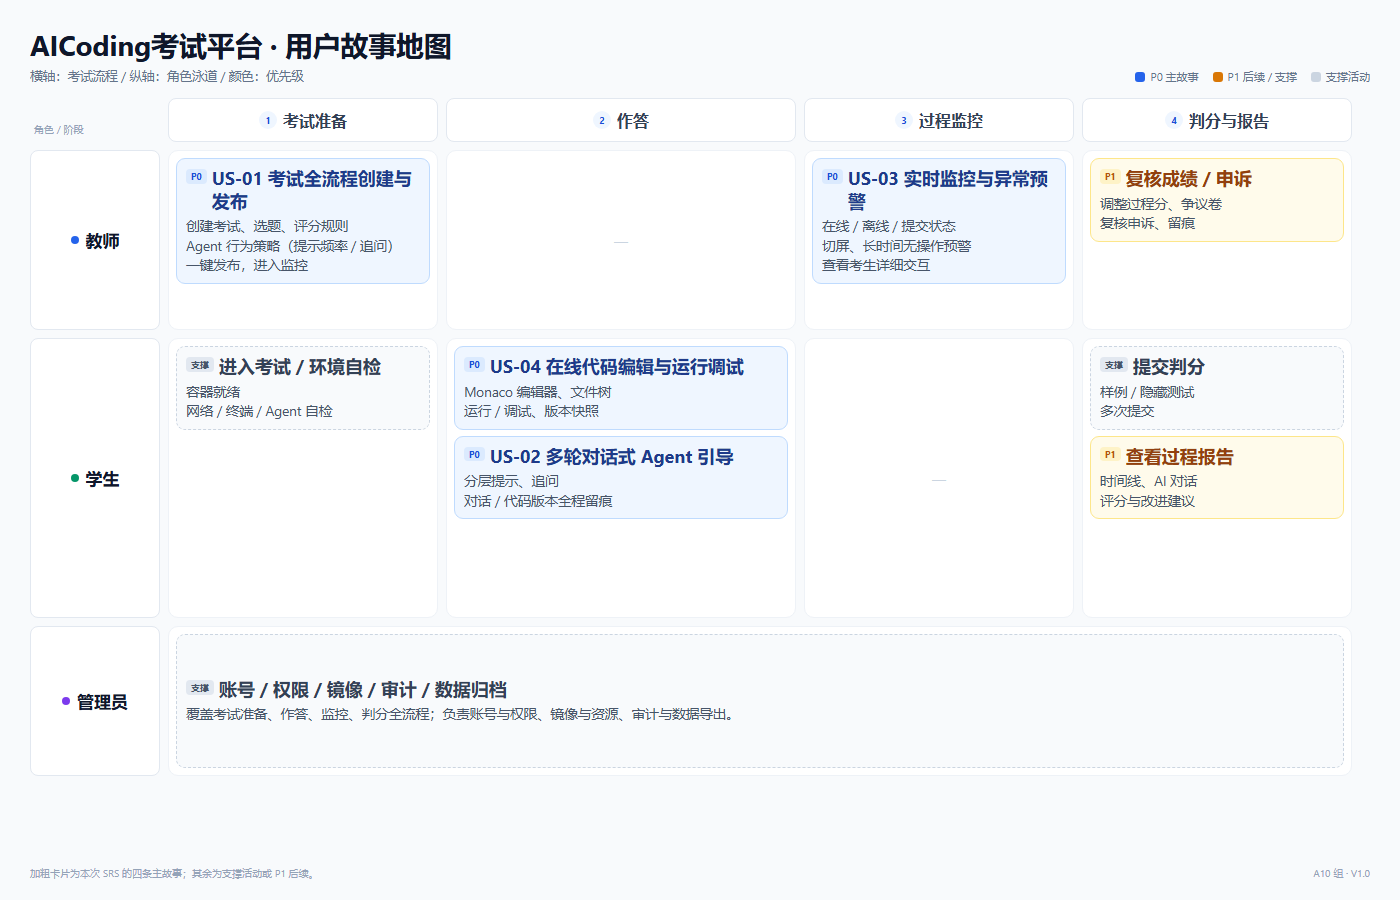
\includegraphics[width=\textwidth]{storymap.png}
\caption{AICoding考试平台用户故事地图}
\label{fig:storymap}
\end{figure}

故事地图按“考试准备—作答—监控—判分—报告”展开，角色泳道和优先级见图。

\subsection{用户故事卡}

\subsubsection*{US-01 考试全流程创建与发布}

\begin{description}[leftmargin=3em,style=nextline,itemsep=2pt]
  \item[角色] 教师（命题人/课程负责人）
  \item[故事] 负责课程考核设计，需要灵活配置考试参数与 Agent 行为策略；通过可视化界面快速创建考试、配置题目与评分规则，一键发布并管理考试全生命周期。
  \item[场景] 教师在考试管理后台，准备为班级创建一次编程考试。
  \item[事件]
  \begin{enumerate}[leftmargin=1.5em,itemsep=1pt]
    \item 教师点击“创建考试”按钮。
    \item 教师填写考试名称、选择题目（从题库或新建）、设定考试时长、配置评分规则与 Agent 行为策略（如提示频率、是否允许追问），保存后发布考试。
    \item 考试发布成功，学生端可见考试入口，教师可进入监控面板。
  \end{enumerate}
  \item[优先级] 高
  \item[难度] 中
\end{description}

\subsubsection*{US-02 多轮对话式 Agent 编程引导}

\begin{description}[leftmargin=3em,style=nextline,itemsep=2pt]
  \item[角色] 考生
  \item[故事] 具备一定编程基础，在考试或训练中遇到思路瓶颈时需要引导而非直接答案；通过与 Agent 多轮对话获得渐进式提示与追问，在不被直接给答案的前提下突破思维卡点，同时交互记录被完整保存用于过程性评分。
  \item[场景] 考生在考试或训练模式下打开编程题目，进入 Agent 交互面板。
  \item[事件]
  \begin{enumerate}[leftmargin=1.5em,itemsep=1pt]
    \item 考生在编码过程中主动点击“请求提示”，或 Agent 检测到长时间无操作后主动发起追问。
    \item 考生与 Agent 进行多轮对话，Agent 根据当前代码状态与题目要求提供分层提示、追问设计思路、引导算法选择；系统实时记录全部对话内容、时间戳与关联代码版本。
    \item 考生关闭对话面板或提交代码，对话记录归档至过程性评分数据池。
  \end{enumerate}
  \item[优先级] 高
  \item[难度] 高
\end{description}

\subsubsection*{US-03 考试过程实时监控与异常预警}

\begin{description}[leftmargin=3em,style=nextline,itemsep=2pt]
  \item[角色] 教师（监考）
  \item[故事] 需要在考试进行中掌握全班考生状态，及时发现异常行为；实时查看考生在线状态、代码提交进度与 Agent 交互频率，对切屏、长时间无操作等异常行为自动预警。
  \item[场景] 考试进行中，教师打开监控面板。
  \item[事件]
  \begin{enumerate}[leftmargin=1.5em,itemsep=1pt]
    \item 教师进入“考试监控”页面，或系统检测到考生异常行为。
    \item 系统展示所有考生的实时状态列表（在线/离线/提交状态），标记异常行为并推送预警通知，教师可点击查看某考生的详细交互记录。
    \item 教师关闭监控面板或考试结束，监控数据自动归档。
  \end{enumerate}
  \item[优先级] 高
  \item[难度] 中
\end{description}

\subsubsection*{US-04 在线代码编辑与多语言运行调试}

\begin{description}[leftmargin=3em,style=nextline,itemsep=2pt]
  \item[角色] 考生
  \item[故事] 需要在浏览器中直接编写、调试和运行代码，无需本地环境配置；获得流畅的在线编码体验，支持多种编程语言（首期 Python 3.11，后续扩展 Java、JavaScript、C++），代码版本变化自动记录。
  \item[场景] 考生在考试或训练模式下打开编程题目，进入代码编辑界面。
  \item[事件]
  \begin{enumerate}[leftmargin=1.5em,itemsep=1pt]
    \item 考生在编辑器中输入或修改代码，点击“运行”或“调试”按钮。
    \item 考生使用在线编辑器编写代码，选择编程语言，执行运行或调试操作，系统返回运行结果并自动保存代码版本快照。
    \item 考生提交代码或保存当前版本，所有版本记录归档至过程性评分数据池。
  \end{enumerate}
  \item[优先级] 高
  \item[难度] 高
\end{description}

\section{系统的总体架构和技术选型}

\subsection{总体架构}

系统采用前后端分离的分层架构，后端以 Python 为主，前端使用 TypeScript/React。浏览器端基于 React 构建三栏式考试工作台（文件树/编辑器、终端/测试输出、Agent 对话面板）；Nginx 作为唯一对外入口，负责 TLS 终止、静态资源服务和 WebSocket 升级转发。应用服务层以 Django + Django REST Framework（DRF）为 API 骨架，Django Channels 处理实时监控所需的 WebSocket 长连接。判题请求不在 HTTP 请求线程中同步执行，而是交给独立的后台判题任务处理；提交后接口立即返回，判题任务完成编译和测试后把结果写回数据库，前端再获取结果。Agent 采用 LangChain 等主流智能体编排框架，支持多智能体框架设计，便于后续进行智能体分级设计。

\subsection{技术选型}

\begin{table}[H]
\centering
\caption{技术选型与理由}
\label{tab:techstack}
\small
\begin{tabularx}{\textwidth}{|p{2.8cm}|p{4.0cm}|Y|}
\hline
\textbf{层次} & \textbf{技术} & \textbf{选型理由} \\ \hline
前端框架 & React 18 + TypeScript & 组件化适合三栏考试工作台的多面板管理，生态成熟，便于与编辑器和终端组件配合。 \\ \hline
代码编辑器 & Monaco Editor & 与 VS Code 同源，提供接近本地 IDE 的语法高亮、补全和错误定位，适合在线答题场景。 \\ \hline
终端 & xterm.js + WebSocket & 浏览器内常用的终端方案，可在网页中执行命令并实时显示输出。 \\ \hline
后端框架 & Django + Django REST Framework & 自带用户、权限和后台管理能力，适合快速搭建考试管理与评分后台；REST 接口便于前后端分离。 \\ \hline
数据库 & MySQL 8.0 & 关系模型适合存放考试、题目、提交和评分等结构清晰的数据，支持事务，保证成绩和状态的一致。 \\ \hline
缓存/队列 & Redis + Celery & Redis 缓存考试状态和监控数据，Celery 把判题放到后台执行，避免提交接口被长时间占用。 \\ \hline
容器/编排 & Docker + Docker Compose & 每位考生一个隔离容器；Compose 统一管理前端、后端、数据库、缓存和判题服务，首期规模下部署简单。 \\ \hline
判题沙箱 & Docker 容器 & 每次判题在独立容器中运行，限制 CPU 和内存，禁止外部网络和特权操作，降低安全风险。 \\ \hline
Agent & LangChain & 较成熟的智能体编排框架，便于组合提示、工具调用和对话流程。 \\ \hline
对象存储 & MinIO & 存放代码快照、判题日志和导出报告等大文件；结构化记录仍放在 MySQL 中。 \\ \hline
部署 & Nginx + Docker Compose + HTTPS & Nginx 统一处理 HTTPS 接入和请求转发，Compose 一键启动整套服务，后续可平滑迁移。 \\ \hline
\end{tabularx}
\end{table}

\subsection{部署方案}

首期采用单机 Docker Compose 部署。所有服务运行在内部网络中，只有 Nginx 映射端口对外提供服务，数据库、缓存、对象存储和判题沙箱都不直接暴露到宿主机。Nginx 负责三件事：HTTPS 接入与跳转、向前端页面提供静态资源、把 API 和实时连接请求转发给后端应用。后端应用以多进程方式运行；判题任务放在独立的后台服务中，可以根据判题负载单独扩容，不影响考试接口的响应。数据库、缓存和对象存储都使用独立数据卷持久化，快照按“考试 / 考生 / 时间”组织存放，便于复核和申诉时查找。


\section{项目的开发迭代计划及后续分工}

\subsection{开发迭代计划}

\begin{table}[H]
\centering
\small
\begin{tabularx}{\textwidth}{|p{1.4cm}|p{2.0cm}|Y|p{3.0cm}|}
\hline
\textbf{轮次} & \textbf{周次} & \textbf{任务} & \textbf{交付物} \\ \hline
第一轮 & 6-7周 & 需求调研（问卷），整体架构设计，实现账号管理和权限分级，题库与测试样例管理& \\ \hline
第二轮 & 8周 & 完成考场核心闭环，实现OJ基本功能& \\ \hline
第三轮 & 9-10周& 接入AI助手服务，完成AI分级权限设计& \\ \hline
第四轮 & 11周& 监考和反作弊功能完善，实现过程性评分细则& \\ \hline
第五轮 & 12-13周& 测试和维护& \\ \hline
收尾 &   14周&  设计使用文档，完善教程& \\ \hline
\end{tabularx}
\end{table}

\subsection{后续分工}

\begin{table}[H]
\centering
\small
\begin{tabularx}{\textwidth}{|p{3.0cm}|p{4.0cm}|Y|}
\hline
\textbf{角色} & \textbf{负责人} & \textbf{职责} \\ \hline
前端 & 石恒睿、李劲逸 & 负责考试工作台、教师后台与墨刀原型落地。 \\ \hline
后端 & 吕浩 & 负责账号权限、考试管理、判题与数据接口。 \\ \hline
Agent & 康祥桢 & 负责 Agent 网关、策略分级、对话留痕与过程数据。 \\ \hline
会议召开 & 康祥桢 & 负责组会安排、会议纪要、进度同步。 \\ \hline
项目管理 & 康祥桢 & 负责里程碑、任务拆分、风险跟踪与对外沟通。 \\ \hline
\end{tabularx}
\end{table}


\subsection{原型链接}

墨刀原型（只读）：\href{https://modao.cc/proto/FgnsjqSBtnggwtjPrLH0B5/sharing}{https://modao.cc/proto/FgnsjqSBtnggwtjPrLH0B5/sharing}

\newpage
\appendix
\section{需求调研记录}

\subsection{问卷概况}
本次问卷共回收 18 份，其中在校学生 17 份、其他 1 份。问卷围绕现有编程考核的不足、AI 编程中的问题、适合的考核任务、重点考察能力、AI 参与方式、评分依据、工作台功能和报告形式展开。

\subsection{主要结果}
\begin{itemize}[leftmargin=2em]
  \item \textbf{现有考核不足。}10/18 选择“主要看最终代码，难以了解分析、修改和验证的过程”；7/18 选择“侧重算法技巧或语法记忆，较少涉及实际项目问题”；4/18 选择“无法充分评价使用 AI 后参与者自身的理解与判断能力”；4/18 选择“没有相关经历，无法判断”。
  \item \textbf{AI 编程问题。}14/18 选择“代码能够运行，但自己难以判断实现是否正确、可靠”；11/18 选择“得到了 AI 生成的代码，却难以解释关键逻辑”；4/18 选择“配置环境或转移 AI 生成的代码占用了较多时间”；3/18 选择“对话、代码修改和测试分散在不同工具中，不便对照和回顾”。
  \item \textbf{适合的考核任务。}修复错误、补充测试、优化代码、扩展功能、审阅代码、拆解需求。
  \item \textbf{重点考察能力。}理解需求与约束、任务拆解、向 AI 提供必要信息并调整要求、识别并纠正 AI 代码中的问题、设计测试或对比实验验证结果、解释关键修改。
  \item \textbf{AI 参与方式。}自主执行、确认后执行、分阶段切换、建议为主。
  \item \textbf{评分依据。}最终代码正确性/测试通过、问题分析与解决步骤、根据 AI 反馈调整、识别并纠正 AI 问题、验证修改与边界情况、解释关键修改。
  \item \textbf{工作台功能。}预配置项目环境、浏览/编辑多文件、AI 结合项目分析修改、展示 AI 修改前后差异并支持采纳/撤销、网页内运行命令/测试、保存阶段版本、显示规则/剩余时间/工具额度。
  \item \textbf{报告形式。}方案对照、结果反馈、能力反馈、过程回顾。
\end{itemize}

\subsection{对需求的启示}
问卷结果支持本产品的三个核心设计：把“最终代码”扩展为“代码 + 过程证据”；把 AI 使用从“禁用/放行”变成可配置、可留痕的协作策略；把工作台和报告做成“环境—编辑—运行—AI 协作—复盘”的闭环。具体功能映射见第 3.3 节。


\end{document}
